
\documentclass[12pt]{article}
%\documentclass[12pt,twocolumn]{article}

\usepackage{listings}
\usepackage{color}
\usepackage{hyperref}
\usepackage[margin=1.0in]{geometry}
\usepackage{graphicx}

\definecolor{dkgreen}{rgb}{0,0.6,0}
\definecolor{gray}{rgb}{0.5,0.5,0.5}
\definecolor{mauve}{rgb}{0.58,0,0.82}

\lstset{%frame=tb,
  language=bash,
  aboveskip=3mm,
  belowskip=3mm,
  showstringspaces=false,
  columns=flexible,
  basicstyle={\small\ttfamily},
  numbers=none,
  numberstyle=\tiny\color{gray},
  keywordstyle=\color{blue},
  commentstyle=\color{dkgreen},
  stringstyle=\color{mauve},
  breaklines=true,
  tabsize=3, 
  postbreak=\raisebox{0ex}[0ex][0ex]{\ensuremath{\color{red}\hookrightarrow\space}}
}

\begin{document}

\title{Framework for Ice Sheet - Ocean Coupled modelling (FISOC) Manual}
\author{Rupert Gladstone (RupertGladstone1972@gmail.com) \and Lenneke Jong \and Ben Galton-Fenzi \and David Gwyther}
%\date{Version 0.2, April 2016}
\maketitle

\newpage 
\tableofcontents
\newpage 

\section{Introduction}

The ``Framework for Ice Sheet - Ocean model Coupling" (FISOC) has been written to enable Ice Sheet Models 
(ISMs) and Ocean Models (OMs) to be run as a single executable to address the co-evolution of ice and ocean 
properties.  
It is primarily designed to handle exchange of variables between ice and ocean at the underside of a floating ice shelf.
At time of writing (5/12/2017) exchange of variables at an ice cliff is 
not supported, though this is a planned development.

In this context an ISM simulates (part of) a marine ice sheet, including both grounded and floating parts, 
representing the dynamic evolution over time of the ice sheet.

An OM simulates the sub-shelf cavity circulation under the floating part of the ice sheet, and optionally also 
a wider ocean domain.

FISOC comprises a set of code modules and driver built using the Earth System Modelling Framework (ESMF, 
\url{https://www.earthsystemcog.org/projects/esmf/}), and written in Fortran 90. 
Some knowledge of the ESMF is essentially in order to fully understand the FISOC code.  It should 
be possible to run FISOC without knowledge of ESMF.
FISOC is intended to be flexible: the additional development effort required to 
couple a different ocean or ice component into the framework is minimal, so 
long as the new component is ESMF-compatible. 

FISOC initially couples the ISM Elmer/Ice to the OM ``Regional Ocean Modelling System'' (ROMS).
A full description of the physical processes represented in FISOC in its 
initial configuration will be described in a GMD paper (this is in 
preparation as of 5/12/2017).

This manual describes how to use FISOC with an ISM and OM for which it has been 
developed (Section~\ref{sec:FISOC_SUG}) and also how to integrate 
additional ISM or OM components 
into the FISOC framework (Section~\ref{sec:FISOC_SDG}).

A number of web links are given at various points in this document.  
The links were correct at the time they were added. 
Please contact the developers if any of these are found to be out of date. 




\section{Installing FISOC with established components}
\label{sec:FISOC_install}

FISOC can be obtained by emailing a request to the developers.  
At the time of writing (5/12/2017) it is maintained and developed in a 
private GitHub repository.  
This will go public when the GMD description paper is 
submitted (inteded in 2018).

FISOC has a simple build process.  The Makefile in the top level FISOC directory contains the 
hard coded dependencies needed to build FISOC code.  The Makefile refers to certain 
environment variables to determine paths and component choices (Section~\ref{sec:EnvVars}). 

Having installed the pre-requisites (Section~\ref{sec:PreReq}), simply run at the command line, 
in the top level FISOC directory:
\begin{lstlisting}
make install
\end{lstlisting}

An example script to build and install FISOC, ``buildFISOCexample.sh'', is available in the top 
level FISOC directory.

FISOC has been built and used with GNU and with Intel compilers. 
This has been carried out on different flavours of Linux. 
The Message Passing Interface (MPI) implementation is OpenMPI. 
In principal it should also work with MPICH, but this has not been tested at time of writing (5/12/2017). 



\subsection{Switching between components}

Many aspects of FISOC are runtime configurable (Section~\ref{sec:FISOC_SUG}), 
but the choice of which component to use is a compile time option, implemented 
by choice of model-specific wrapper. 
This is determined by environment variables FISOC\_OM and FISOC\_ISM 
(Section~\ref{sec:EnvVars}). 

In order to test the build the dummy wrappers may be used. 
Libraries are not needed for dummy wrappers, and the corresponding 
environment variables can be set to any value.
See  ``buildFISOCexample.sh'' for examples. 

In addition to the dummy wrappers, undocumented ISM components 
(as of 5/12/2017) include: 
``FOrcing OffLine'' (FOOL), which acts as a wrapper for netcdf files 
containing time evolving geometry forcing we want to use to force the 
OM; 
``Frank's Ice Shelf model'' (FISh), a very simple flowline SSA 
ice shelf model from Frank Pattyn, used for simple testing during 
development.



\subsection{FISOC Environment Variables}
\label{sec:EnvVars}

Several environment variables may be used in the build process. 
Some of these are mandatory. 
Variables listed as optional here may be mandatory for some configuratons 
other than ``dummy''.
These environment variables are not used at run time, only during 
the compilation/installation of FISOC.


\begin{flushleft}
\textbf{ESMFMKFILE}                                \\ 
Required.                                          \\
Tells FISOC where to find key ESMF information.    \\
\vspace{6pt}
\textbf{FISOC\_INSTALL\_DIR}                       \\ 
Optional.                                          \\
Determines where the FISOC executable will be installed. Defaults to \$HOME/bin. 
The user should also ensure this location is in their \$PATH. \\
\vspace{6pt}
\textbf{FISOC\_EXE}                                \\ 
Optional.                                          \\
Name of the FISOC executable.  Defaults to FISOC\_caller. \\
\vspace{6pt}
% now set through cpp flags
%\textbf{FISOC\_MPI}                                \\ 
%Optional. Possible value ``yes''.                  \\
%Sets preprocessor flag to tell FISOC whether this is a parallel compilation.
%Defaults to serial.                                \\
%\vspace{6pt}
\textbf{FISOC\_OM}                                 \\ 
Required. Possible values ``dummy'', ``ROMS''.     \\
Determines which OM component will be used.        \\
\vspace{6pt}
\textbf{FISOC\_OM\_INCLUDE}                         \\ 
Optional.                                           \\
Specifies the path where the OM header files are located.\\
\vspace{6pt}
\textbf{FISOC\_OM\_LIBPATH}                         \\
Optional.                                           \\
Specifies the path where the OM library files are located.\\
\vspace{6pt}
\textbf{FISOC\_OM\_LIBS}                            \\
Optional.                                           \\
Specifies the linker directives needed to link the OM library to FISOC. \\
\vspace{6pt}
\textbf{FISOC\_ISM}                                 \\
Required. Possible values ``dummy'', ``Elmer'', ``FISh'', ``FOOL''.     \\
Determines which ISM component will be used.        \\
\vspace{6pt}
\textbf{FISOC\_ISM\_INCLUDE}                        \\ 
Optional.                                           \\
Specifies the path where the ISM header files are located.\\
\vspace{6pt}
\textbf{FISOC\_ISM\_LIBPATH}                        \\
Optional.                                           \\
Specifies the path where the ISM library files are located.\\
\vspace{6pt}
\textbf{FISOC\_ISM\_LIBS}                           \\
Optional.                                           \\
Specifies the linker directives needed to link the ISM library to FISOC. \\
\vspace{6pt}
\textbf{CPPFLAGS}                                   \\
Optional.                                           \\
Preprocessor directives may be specified here.  
Preprocessor directives used by FISOC:              \\
\textbf{FISOC\_MPI}                                 \\ 
Should be defined for parallel compilation but not for 
serial compilation.  Activates code sections specific to parallel simulations. 
At time of writing (5/12/2017) serial compilation has not been recently tested
and may or may not work.                            \\
%\vspace{6pt}
See also Section~\ref{sec:PreReqROMS} for ROMS-specific preprocessor directives.
\end{flushleft}



\subsection{Pre-requisites}
\label{sec:PreReq}

A Message Passing Interface (MPI) implementation, such as 
OpenMPI is required.\\
 \url{http://www.open-mpi.org/}

The Network Common Data Form (NetCDF) Fortran interface must be available. 
More specifically, NetCDF4 in parallel should be used (this is not the same as PnetCDF). \\
\url{http://www.unidata.ucar.edu/software/netcdf/}

ESMF must be available. ESMF should have been built with NetCDF and MPI 
(see also notes in Appendix~\ref{app:A}). \\
\url{https://www.earthsystemcog.org/projects/esmf/}.

%For example, environment variables like these may be used for the ESMF build
%\begin{lstlisting}
%export ESMF_NETCDF="split"
%export ESMF_NETCDF_INCLUDE="/usr/local/include/"
%export ESMF_COMM="openmpi"
%\end{lstlisting}

Viable ISM and OM components must be available for any physically meaningful simulations
(the build may be tested using ``dummy'' components).  
See Sections~\ref{sec:PreReqElmer} and \ref{sec:PreReqROMS}.


\subsubsection{Elmer/Ice}
\label{sec:PreReqElmer}

\textbf{Compiling Elmer/Ice for FISOC} \\
At time of writing (5/12/2017) FISOC requires a non-standard Elmer/Ice 
code branch. 
The Elmer repository is here:
\url{https://github.com/ElmerCSC/elmerfem/}.
The standard branch used by glaciologists is the elmerice branch. 
The branch needed for FISOC is the elmerice\_FISOC branch. 
It is intended to merge the changes in 2018.
You can checkout the relevant branch with a command like this:
\begin{lstlisting}
git clone git://www.github.com/ElmerCSC/elmerfem -b elmerice_FISOC MyLocalName
\end{lstlisting}

There is nothing FISOC-specific about the Elmer/Ice build process.  
So long as you have the FISOC-compatible code branch, you can build Elmer/Ice 
just the same as normal. 
The Elmer/Ice wiki has information on a standard build:
\url{http://elmerice.elmerfem.org/wiki/doku.php?id=compilation:compilationcmake}

\vspace{10pt}

\textbf{Compiling FISOC with Elmer/Ice}\\
When compiling FISOC with Elmer/Ice, FISOC needs to know where to 
find the relevant Elmer/Ice libraries.  
This can be done at FISOC compile time through the 
\$FISOC\_ISM
environment variables.  For example:

\begin{lstlisting}
export FISOC_ISM="Elmer"
export FISOC_ISM_INCLUDE="$ELMER_HOME/share/elmersolver/include"
export FISOC_ISM_LIBPATH="$ELMER_HOME/lib/"
export FISOC_ISM_LIBS="-lelmersolver"
\end{lstlisting}





\subsubsection{ROMS}
\label{sec:PreReqROMS}

\textbf{Compiling ROMS for FISOC} \\
FISOC has been developed and tested with an ice shelf enabled version of ROMS. 
This is branched from the Rutgers ROMS repository.  Information about the Rutgers ROMS 
can be found at \url{https://www.myroms.org/}.

Development of the ice shelf enabled version  is currently ongoing 
in a private repository 
(please contact the developers if you need access to this).
A public version of the ice shelf enabled version is also available 
through github: 
\url{https://github.com/bkgf/romsIceShelf}.  
Please use the ``FISOC\_friendly'' branch.
At time of writing (5/12/2017) the public version is out of date and 
the private version should be used. 
It is intended to push changes to the public version at the time of 
submission of the FISOC GMD paper, during 2018.

Example build scripts can be found in the ROMS/Bin subdirectory of a git clone 
from the repository mentioned above.
It is assumed that users are familiar with a standard ROMS build process. 


When compiling ROMS for use with FISOC, the following additional environment
variables are needed:
\begin{lstlisting}
export MAKE_SHAREDLIB="Yes"
export LIBDIR="/usr/local/lib"
export MY_CPP_FLAGS=" -DFISOC"
\end{lstlisting}

It is essential to activate the option to compile the ROMS shared library, which 
is done by setting the environment variable MAKE\_SHAREDLIB to any value. 
The -fPIC flag is essential, and this will in general be activated 
by MAKE\_SHAREDLIB in a makefile supplement included by a line like 
this in the makefile:
\begin{lstlisting}
include $(COMPILERS)/$(OS)-$(strip $(FORT)).mk
\end{lstlisting}
This should simply work, but may require minor modifications on new 
OS/compiler combinations.

The shared library will be installed in the location given by the 
 LIBDIR environment variable. 

The -DFISOC flag activates FISOC-specific code segments.  
This includes telling ROMS to use a 
specific hard coded unit rather than outputting to screen.  This relies on the 
same unit being hard coded in the FISOC ROMS wrapper, and results in the ROMS 
messages being sent to file instead of printed to screen.

Some aspects of the ROMS setup for specific simulations are determined at 
compile time rather than run time. 
These are determined through cpp directives set in an application-specific 
header file in ROMS/Include in the ROMS clone. 
ROMS must be compiled with an ``application'' (this is set through an 
environment variable, see example ROMS build script) that has been setup for 
use with FISOC. 
This should give a good indication of which applications are FISOC-compatible:
\begin{lstlisting}
grep ``ifdef FISOC'' ROMS/Include/*h
\end{lstlisting}

The cpp options are described in ROMS/Include/cppdefs.h. 
More detail of the FISOC specific options is given below, but to compile ROMS 
for use with 
existing FISOC examples, knowledge of these is not required as the header 
files will set the required cpp directives and the header file is determined by 
choice of ROMS application.

\begin{flushleft}
To tell ROMS to expect FISOC to provide a cavity change rate:\\
FISOC\_DDDT\\
To tell ROMS to expect FISOC to provide an upper ice surface change rate
(at time of writing, 5/12/2017, this is required for grounding line migration 
and is used to update the wet/dry masks based on floatation):\\
FISOC\_DSDT\\
To tell ROMS to expect FISOC to directly overwrite the iceshelf draft 
(this and FISOC\_DDT are mutually exclusive):\\
FISOC\_DRAFT\\
To tell ROMS to expect to receive a vertical temperature gradient 
at the ice base from FISOC: \\
FISOC\_DTDZ\\
To tell ROMS to calculate the averages of the variables provided to FISOC at 
the end of each ROMS run call:\\
ROMS\_AVERAGES\\
If ice shelf geometry evolution is required in ROMS this options must be 
defined:\\
ICESHELF\_MORPH\\
If grounding line movement is required in ROMS the following cpp options 
must be defined:\\
LIMIT\_BSTRESS\\
LIMIT\_ICESTRESS\\
WET\_DRY
\end{flushleft}


By default ROMS will install the module files in the directory given by 
 SCRATCH\_DIR.  

\vspace{10pt}
\textbf{Compiling FISOC with ROMS}\\
When compiling FISOC with ROMS, FISOC needs to know where to 
find the relevant ROMS libraries.  
This can be done at FISOC compile time through the 
\$FISOC\_OM
environment variables.  For example:

\begin{lstlisting}
export MY_ROMS_DIR="/home/elmeruser/Source/ROMSIceShelf_devel"
export FISOC_OM="ROMS"
export FISOC_OM_LIBS="-loceanM"
export FISOC_OM_INCLUDE="${MY_ROMS_DIR}/Build"
export FISOC_OM_LIBPATH="/usr/local/lib"
\end{lstlisting}

%ROMS uses C preprocessor (cpp) directives to determine which parts of the code are compiled, 
%and these may vary across experiments, requiring ROMS to be compiled multiple times. 
The ROMS cpp directives require matching cpp directives in the FISOC 
compilation process. 
These can be set for a FISOC build using the CPPFLAGS environment variable.
For example (see also the example FISOC build script):
\begin{lstlisting}
export CPPFLAGS="$CPPFLAGS -D ROMS_DRAFT"
\end{lstlisting}
At the time of writing, the relevant values are ROMS\_MASKING, ROMS\_SPHERICAL, 
ROMS\_DDDT, ROMS\_DSDT, ROMS\_DRAFT and ROMS\_AVERAGES. Use of the averaged melt rate from ROMS is activated in FISOC by the ROMS\_AVERAGES cpp. The general rule is that any of these directives that 
are defined for the ROMS compilation need to be defined also for the FISOC 
compilation. 




% put this in GMD paper?

%Setting FISOC\_DSDT activates the following in ROMS:

%In the same way that zice is added to the GRID type and used to indicate height of the lower surface of the iceshelf relative to sea level (i.e. iceshelf draft), sice is added to the GRID type to indicate height of the upper surface of the ice sheet/shelf. sice can be read from netcdf in the same was as zice.

%In the same way that iceshelf\_dddt is added to the ICESHELFVAR type and accessed from FISOC to set the rate of change of iceshelf draft wrt time, iceshelf\_dsdt is added to ICESHELFVAR to set the rate of change of sice with time.  If FISOC does not update iceshelf\_dsdt then the upper ice surface will remain static.

% The value for ice density (and a couple other things?) defined in iceshelf\_mod.h is used (overwrite these from FISOC?)


%\subsection{Troubleshooting}







\section{Running FISOC}
\label{sec:FISOC_SUG}

The FISOC executable is by default called FISOC\_caller, and should be located in your 
path after installation. 
The installation is specific to the choice of component (you need to re-compile if you switch, for 
example, from one ISM to another).  
Beyond choice of components, all run time choices are made in the FISOC\_config.rc file
(Section~\ref{sec:config}), 
or through component specific initialisation.

For example, you can run FISOC in serial like this:
\begin{lstlisting}
FISOC_caller
\end{lstlisting}
You can run FISOC in parallel like this (depending on your system):
\begin{lstlisting}
mpirun -np 4 FISOC_caller
\end{lstlisting}

In the first instance a dummy coupler can be run be setting both environment variables FISOC\_ISM and 
FISOC\_OM to ``dummy'' at compile time.  This can help to test the compilation, and was used during development, 
but performs no meaningful science.  

In verbose mode (Section~\ref{sec:config}) some run time information may be printed to the screen.  
Independently of this, log files are always written (see below). 






\subsection{FISOC output files}


The outputs from FISOC include: \\
1. Standard out from the job.  In interactive runs it is written to the screen. \\
2. Standard out from the ice model.  This is redirected to a file named in the FISOC\_config file. \\
3. Standard out from the ocean model.  This is redirected to a file named in the FISOC\_config file. \\
4. ESMF log files (usually named PET*.log). 

FISOC can output basic netcdf files from the OM generic wrapper 
on the OM grid. 
FISOC can do this for both ISM and OM variables.
This capability is mainly recommended just for sanity checking.

%The ISM and OM have their standard out directed to files named in the 
%FISOC\_config.rc file. 
%At time of writing (5/12/2017) ROMS stdout is not correctly implemented and sometimes 
%writes to fort.31.

FISOC log files have default filenames of ``PET\#.FISOC.Log'', where ``\#'' is a number from 0 upwards 
indicating the ``Persistent Execution Thread'' (PET). 
These logs are created by FISOC/ESMF and contain run time messages and errors that can 
be helpful with troubleshooting.
Note that by default FISOC appends to the logs rather than over-writing at run time, so you may wish to delete 
old logs periodically. 

Aside: PET is an ESMF abstraction designed to be general over differing parallel implementations. 
In FISOC, there is always a 1:1 relationship between PETs and MPI processes. 






\subsection{FISOC runtime configuration}
\label{sec:config}

The FISOC config file is named FISOC\_config.rc, and is expected to be present 
in the current directory when running FISOC.  
This is a resource file, as described by the 
ESMF documentation.  It supports different types and also lists. 
In principle, lists of mixed types are supported, though FISOC does not utilise this capability.
Basic syntax highlighting for .rc files can be activated within emacs 
(see notes in doc/FISOC\_emacsMode.asc in the FISOC repository).

FISOC\_config.rc mainly contains parameters specific to the coupling rather than to the running of 
individual components.  
Components should use their standard means for configuration, and component-specific configuration files 
should be specified in the FISOC configuration file.

Some of the FISOC config entries are strictly required and some are optional.
This section describes all the valid standard config entries. 
Note that model-specific non-standard entries can be added if needed, and use of these 
should be through the model-specific wrapper code.


\begin{flushleft}
%\textbf{label:}               [TYPE]   [Required?]                         \\
%Description                                                                \\
%\vspace{6pt}
%\vspace{6pt}
%\textbf{ISM\_meshFile:}       [STRING] [optional]                          \\
%The name of a netcdf file containing the ISM mesh in ESMF format.          \\
%\vspace{6pt}
\textbf{\underline{ISM options}} \\
\vspace{6pt}
\textbf{ISM\_configFile:}     [STRING] [optional]                          \\
The name of the ISM-specific config file.                                  \\
\vspace{6pt}
\textbf{ISM\_stdoutFile:}     [STRING] [optional]                          \\
The name of a file to which to write the ISM standard output.  May be 
required depending on model-specific wrapper.                              \\
\vspace{6pt}
\textbf{FISOC\_ISM\_ReqVars:} [STRING] [required]                          \\
List of variable names required to be provided by the ISM.                 \\
\vspace{6pt}
\textbf{ISM\_varNames:} [STRING] [optional]                                \\
List of native names of variables in the ISM, for use by the model-specific 
wrapper.  May also be required or unused depending on the wrapper. Must be 
same length as \textbf{FISOC\_ISM\_ReqVars}.                               \\
\vspace{6pt}
\textbf{FISOC\_ISM\_DerVars:} [STRING] [required]                          \\
List of variables derived by FISOC from the ISM variables. These are 
calculated from ISM required variables by hard coded routines in 
FISOC\_ISM or FISOC\_utils. This list is allowed to be empty.              \\
\vspace{6pt}
\textbf{ISM\_maskOMvars:} [LOGICAL] [optional]                             \\
Determines whether the ISM\_maskOMvars should be turned on or not. The generic
pre-requisite for this is that ISM\_gmask must be present, i.e. it must be a 
member of either FISOC\_ISM\_ReqVars or FISOC\_ISM\_DerVars.
The Elmer-specific pre-requisite is that the Elmer variable GroundedMask must
exist according to the .sif.
\vspace{6pt}
\textbf{ISM\_gridType:}        [STRING] [required]                          \\
Which ESMF object to use.  Valid values are ESMF\_mesh (typically used 
o describe unstructured meshes) and ESMF\_grid (typically used to 
describe structured grids, supports stagered grids).                       \\
\vspace{6pt}
\textbf{ISM2OM\_vars:}        [STRING] [optional]                          \\
List of variables to be passed from the ISM to the OM. Defaults to 
all ISM variables (union of required and derived variables). If an empty 
list is given no variables will be passed from the ISM to the OM.  This 
can be useful for unit testing.                                            \\ 
\vspace{6pt}
\textbf{ISM2OM\_init\_vars:}  [LOGICAL] [optional]                         \\
Determines whether the ISM2OM\_vars should be passed to the OM during the 
second phase of OM initialisation.   Default is .TRUE.                     \\ 
\vspace{6pt}
\textbf{ISM2OM\_regrid:}       [STRING] [optional]                         \\
The ESM regridding method to use.  If not set, the default will be 
written to the log files.  Possible values are given in the ESMF 
documentation. 
\url{http://www.earthsystemmodeling.org/esmf_releases/public/last/ESMF_refdoc/node9.html#SECTION090146000000000000000}

\vspace{22pt}

\textbf{\underline{OM options}} \\
\vspace{6pt}
\textbf{OM\_configFile:}      [STRING] [optional]                          \\
The name of the ISM-specific config file.                                  \\
\vspace{6pt}
\textbf{OM\_stdoutFile:}     [STRING] [optional]                           \\
The name of a file to which to write the OM standard output.  May be 
required depending on model-specific wrapper.                              \\
\vspace{6pt}
\textbf{FISOC\_OM\_ReqVars:}  [STRING] [required]                          \\
List of variable names required to be provided by the OM.                  \\
\vspace{6pt}
\textbf{OM\_ReqVars\_stagger:} [STRING] [optional]                         \\
Corresponding exactly to \textbf{FISOC\_OM\_ReqVars}, descriptions of the 
grid stagger for each variable.                                            \\
\vspace{6pt}
\textbf{FISOC\_OM\_DerVars:}  [STRING] [required]                          \\
List of variables derived by FISOC from the OM vars.  
To be calculated from OM vars by hard coded routines in FISOC\_OM.        \\
\vspace{6pt}
\textbf{OM\_gridType:}        [STRING] [required]                           \\
Which ESMF object to use.  Valid values are ESMF\_mesh and ESMF\_grid.     \\
\vspace{6pt}
\textbf{OM2ISM\_vars:}        [STRING] [optional]                          \\
List of variables to be passed from the OM to the ISM. Defaults to 
all OM variables (union of required and derived variables). If an empty 
list is given no variables will be passed from the OM to the ISM.  This 
can be useful for unit testing.                                            \\ 
\vspace{6pt}
\textbf{OM2ISM\_init\_vars:}  [LOGICAL] [optional]                         \\
Determines whether the OM2ISM\_vars should be passed to the ISM during the 
second phase of ISM initialisation.   Default is .TRUE.                    \\ 
\vspace{6pt}
\textbf{OM2ISM\_regrid:}       [STRING] [optional]                         \\
The ESMF regridding method to use.  If not set, the default will be 
written to the log files.  Possible values are given in the ESMF 
documentation. 
\url{http://www.earthsystemmodeling.org/esmf_releases/public/last/ESMF_refdoc/node9.html#SECTION090146000000000000000}                                        \\
\vspace{6pt}
\textbf{OM\_initCavityFromISM:}  [LOGICAL] [optional]                      \\
Switch to allow the OM to overwrite its cavity geometry with ISM\_z\_l0 
during the second phase of initialisation.
Defaults to .FALSE.                                                        \\
\vspace{6pt}
\textbf{OM\_cavityUpdate:}   [STRING] [optional]                           \\
How to process ISM ice draft for use in OM.  Valid values are RecentIce    \\
(default), Rate, CorrectedRate, and Linterp.                               \\
\vspace{6pt}
\textbf{OM\_WCmin:}  [REAL] [optional]                                     \\
Minimum water column thickness imposed by OM.  Defaults to zero.  When 
using ROMS, this corresponds to the ROMS DCRIT (in the ,in file) and 
should be set to the same value.  Only used with CorrectedRate to 
preserve a ``dry'' water column under grounded ice.                        \\
\vspace{6pt}
\textbf{OM\_CavCorr:}  [REAL] [optional]                                   \\
The proportion of the OM - ISM cavity discrepancy to correct for in one 
FISOC call to the  OM run method.  Defaults to 0.2.  Only used with 
CorrectedRate.                                                             \\
\vspace{6pt}
\textbf{OM\_outputInterval:} [INTEGER][optional]                           \\
FISOC collects OM output once every OM\_outputInterval OM timesteps. 
Defaults to 1.  dt\_ratio/OM\_outputInterval must be integer.              \\
\vspace{22pt}


\textbf{\underline{Netcdf output options}}                                 \\
Note: these are considered OM options because the output writing occurs 
from the OM generic wrapper.  The OM import state here contains the 
ISM variables regridded to the OM grid.                                    \\
\textbf{OM\_writeNetcdf:}   [LOGICAL] [optional]                           \\
Switch for dumping the OM import and export variables to NetCDF files.
Defaults to .TRUE.                                                         \\
\vspace{6pt}
\textbf{output\_dir:}  [STRING] [optional]                                 \\
Path to directory (must already exist) to which to write the NetCDF files. 
Defaults to current directory.                                             \\
\vspace{6pt}
\textbf{OM\_NCfreq:}  [STRING] [optional]                                 \\
Output writing frequency.
Defaults to ``all''.  Valid values are ``all'' or ``ISM'' (only write 
netcdf outputs after an ISM timestep).
\vspace{22pt}

\textbf{\underline{Timestepping options}}                                  \\
\textbf{OM\_dt\_sec:}         [INTEGER][required]                          \\
OM timestep length in seconds.  When using ROMS, this may be a multiple 
of the ROMS timestep length, in which case each FISOC call to the ROMS 
run method will run multiple ROMS timesteps.                               \\
\vspace{6pt}
\textbf{dt\_ratio:}          [INTEGER][required]                           \\
ISM/OM timestep ratio.                                                     \\
\vspace{6pt}
\textbf{start\_year:}        [INTEGER][required]                           \\
Start year and month define the start time of the coupled simulation.      \\
\vspace{6pt}
\textbf{start\_month:}       [INTEGER][required]                           \\
\vspace{6pt}
\textbf{end\_year:}          [INTEGER][optional]                           \\
End year and month define the finish time of the coupled simulation.       \\
\vspace{6pt}
\textbf{end\_month:}         [INTEGER][optional]                           \\
\vspace{6pt}
\textbf{runLength\_ISM\_steps:} [INTEGER][optional]                        \\
As an alternative to specifying an end time, the run length in terms of 
ISM timesteps may be specified.                                            \\
\vspace{22pt}

%after adding atmos model...
%    "FISOC_dt_sec" "AM_ts" "OM_ts" "ISM_ts"
%    "AO_cpl_ts" "AIS_cpl_ts" "OIS_cpl_ts"

\textbf{\underline{General options}}                                       \\
\textbf{verbose\_coupling:}  [LOGICAL][required]                           \\
If true, some run time information is printed to the screen.  
A log file is always 
written, but writing to the log during timestepping is suppressed when 
verbose\_coupling is false.\\
\end{flushleft}



\subsubsection{FISOC variables}
\label{sec:FISOCvars}

The union of \textbf{FISOC\_ISM\_ReqVars}, \textbf{FISOC\_ISM\_DerVars}, \textbf{FISOC\_OM\_ReqVars} 
and \textbf{FISOC\_OM\_DerVars} describes the full set of variables required by FISOC for a given simulation. 
Valid values are given in Table~\ref{tab:vars}.
Note that the units given in Table~\ref{tab:vars} are suggested units.  FISOC doesn't care about units, but 
the user must ensure unit consistency.  There may be hard coded unit assumptions in the model specific 
wrappers.

Note: dBdt is probably not a suitable choice for ice shelf basal melt rate.  
Simply m (i.e. full name OM\_m) would probably be better, to avoid confusion with dddt 
(rate of change of ice draft).

\begin{table}
  \begin{center}
    \begin{tabular}{ l|l|l }
      Variable              & Description                                  & Units \\
      \hline
      ISM\_temperature\_l0  & Ice temperature at the ice ocean interface.  & K \\
      ISM\_temperature\_l1  & Ice temperature in the ISM one level above   & K \\
                            & the ice ocean interface.                     &   \\ 
      ISM\_z\_l0            & Height relative to sea level of the ice      & m \\
                            & base.                                        &   \\
      ISM\_z\_lts           & Height relative to sea level of the ice      & m \\
                            & top surface.                                 &   \\
      ISM\_z\_l1            & Height relative to sea level of the first    &   \\
                            & ISM model level above the ice base.          & m \\
      ISM\_z\_l0\_previous  & Height relative to sea level of the ice      & m \\
                            & base one ISM timestep previously.            &   \\
      ISM\_z\_lts\_previous & Height relative to sea level of the ice      & m \\
                            & top surface one ISM timestep previously.     &   \\
      ISM\_thick            & Ice thickness                                & m \\
      ISM\_dTdz\_l0         & Vertical temperature gradient in the ice     & K/m \\
                            & at the ice base.                             &   \\
      ISM\_dddt             & Rate of change of the ice draft with respect & m/a \\
                            & to time.                                     &   \\
      ISM\_dsdt             & Rate of change of the ice top surface        & m/a \\
                            & height with respect to time.                 &   \\
      ISM\_velocity\_l0     & Ice flow velocity at the ice base            & m/a \\
      ISM\_maskOMvars       & Mask the fields being passed from OM         &   \\
                            & to the ISM                                   &   \\
      OM\_dBdt\_l0          & Ice shelf basal melt rate.                   & m/a \\
      OM\_temperature\_l0   & Ocean temperature at the ice ocean           &   \\
                            & interface.                                   &   \\
    \end{tabular}
  \end{center}
  \caption{FISOC standard variables and typical units.  
    Note that heights relative to sea level are always positive upward.}
  \label{tab:vars}
\end{table}

As a naming convention, ``z'' refers to the vertical coordinate, and ``l0'' and ``l1'' refer to the 
model level at the ice-ocean interface (this would typically be the lowest level of the ISM or 
the uppermost level of the OM) and one level above it, respectively. ``lts'' refers to the top 
surface of the ISM.

FISOC outputting occurs on the ocean grid, and consists of dumping both the import and 
export fields to netcdf files. 
\textbf{FISOC\_ISM\_ReqVars} may contain variables that are required only so that they can be written 
out on the ocean grid (typically as a sanity or regridding check) rather 
than actually being needed by the OM.

The list of derived variables, \textbf{FISOC\_ISM\_DerVars}, indicates which variables are needed by the 
OM but are not calculated by the ISM or its wrapper. 
The methods for calculating the derived variables are hard coded in FISOC\_ISM.f90. 
Valid values for  \textbf{FISOC\_ISM\_DerVars} include:

ISM\_z\_l0\_previous.  This is the depth of ice base at previous ISM timestep. This is simply stored 
in memory.  No calculation is required, but this variable is needed for the other ``derived'' variables. 

ISM\_dTdz\_l0.  Temperature gradient at ice base.  This is calculated as 
\begin{equation}
ISM\_dTdz\_l0 = \frac{ISM\_temperature\_l1 - ISM\_temperature\_l0}{ISM\_z\_l1 - ISM\_z\_l0}
\end{equation}

ISM\_dddt.  Rate of change of depth of ice base.  This is calculated as 
\begin{equation}
ISM\_dddt = \frac{ISM\_z\_l0 - ISM\_z\_l0\_previous}{ISM\_dt}
\end{equation}

ISM\_dsdt is calculated similarly to ISM\_dddt.

Not all ISM variables need to be passed to the OM, and vice versa.  
This choice is made by the 
user through use of configuration options ISM2OM\_vars and OM2ISM\_vars.  
These options alow the user to specify a subset of the full set of 
required and derived variables that will be passed to the other component 
in a given simulation.  An empty list can be used to avoid any variables 
being passed between components.  This can be useful during testing and 
troubleshooting.

A note on efficiency (relevant on 5/12/2017): 
All the ISM and OM variables are currently being regridded and passed 
to the wrapper for the opposite component.  It is at the model-specific 
wrapper level that ISM2OM\_vars and OM2ISM\_vars are checked.  If regridding 
becomes a significant proportion of FISOC's computational cost this 
should be re-implemented to reduce non-essential regridding operations.





\subsubsection{Updating the ice shelf cavity for the OM}

Several options are available through FISOC for updating the OM representation 
of the ocean cavity. 
These vary from the simplest option of using 
the most recent cavity geometry from the ISM to update the OM representation of 
cavity geometry to smoother options via either interpolation in time or 
specifying a rate of change of cavity geometry.

The options (summarised in Table~\ref{tab:cavity}) are all implemented 
within FISOC, based on the cavity geometry 
calculated by the ISM.  
Some options are through FISOC derived variables, as described 
in Section~\ref{sec:FISOCvars}.  
The key ISM output from which all cavity options 
are calculated is ISM\_z\_l0.  

\begin{table}
  \begin{center}
    \begin{tabular}{ llll }
      Cavity option  & Summary                                    & Required ISM2OM \\
                     &                                            &  variable       \\
      \hline
      RecentIce      & Most recent ice draft from ISM             & ISM\_z\_l0      \\
      Rate           & Rate of change of ice draft from two most  & ISM\_dddt       \\
                     & recent ISM steps                           &                 \\
      CorrectedRate  & As above with additional drift correction  & ISM\_dddt       \\
      Linterp        & Time-interpolated ice draft from two most  & ISM\_z\_l0\_linterp \\
                     &  recent ISM steps                          &                  \\
    \end{tabular}
  \end{center}
  \caption{
    Cavity update options.  Note that of the possible ISM cavity variables 
    (ISM\_z\_l0, ISM\_z\_l0\_linterp, ISM\_dddt) only the required variable 
    (third column) should be passed to the OM (constrained using ISM2OM\_vars).
    At time of writing (5/12/2017) the Rate and CorrectedRate are giving 
    the most reliable outcomes and are recommended.
  }
  \label{tab:cavity}
\end{table}

The FISOC GMD paper will provide more  details about these approaches 
to updating the ocean 
representation of the ice shelf cavity, and also about the wetting and 
drying scheme used for grounding line migration.




\subsubsection{Grids and meshes}
OM\_gridType and ISM\_gridType refer to the type of ESMF object to be used for holding information about 
the model grid.  Typically models utilising unstructured meshes (e.g. Elmer/Ice) would use an 
ESMF\_mesh object for holding mesh information in FISOC and models utilising structured grids 
(e.g. ROMS) would use an ESMF\_grid object for holding grid information in FISOC.








\subsection{Timestepping}

Different asynchronous timestepping options are planned.
Currently recommended (6/12/2017) is to set dt\_ratio = 1 and use the 
ISM timestep for both the ISM and OM components. 
ROMS will run as many timesteps as it needs to (see DT in the ROMS .in file) 
for each call to the ROMS run method. 
With this approach the Rate or CorrectedRate methods for cavity evolution 
are recommended. 
FISOC can pass the ROMS melt rate to the ISM after the call to the 
ROMS run method. 
It might be preferable to get ROMS to provide an average rather than a final 
snapshot for the melt rate. This should be straightforward but is NYI.

%***fill in this section we've implemented both tight coupling (ice and ocean both running 
%on the same timescale) and loose coupling (for longer time scales where the ocean is run 
%to steady state then the ice sheet continues until significant change has occurred in the cavity).




\subsection{Parallelism}

ESMF supports any combination of concurrent and or sequantial parallelisation. 
FISOC is currently (6/12/2017) set up for sequential coupling, where the 
full set of processors are used first for the ISM call then for the OM call. 
It should not be too hard to implement something more flexible if needed 
in the future.



\subsection{Running FISOC with Elmer/Ice} 
For dynamic linked libraries, shared object files may be needed at run time.  
This can be ensured through use of 
the \$LD\_LIBRARY\_PATH environment variable. 

For example (it is assumed \$ELMER\_HOME was set during Elmer installation):
\begin{lstlisting}
export LD_LIBRARY_PATH="$FISOC_ISM_LIBPATH/:$LD_LIBRARY_PATH"
\end{lstlisting}

As with a normal Elmer/Ice simulation, the mesh should be partitioned into the 
same number of partitions as the number of processors (which is the same as the number of 
ESMF PETs and DEs, but don't worry if you don't know what those things are). 

More information about Elmer, and especially Elmer/Ice, can be found on several sources 
on the internet.

\begin{flushleft}
\url{https://www.csc.fi/web/elmer}\\
\url{http://www.nic.funet.fi/pub/sci/physics/elmer/doc/}\\
\url{http://elmerice.elmerfem.org/}\\
\url{http://elmerice.elmerfem.org/wiki/doku.php}\\
\url{http://www.elmerfem.org/forum/}\\
\end{flushleft}



\subsubsection{Elmer/Ice specific configuration}

The following options in the FISOC configuration file are used by Elmer/Ice.  These 
are non-standard configuration options.

\begin{flushleft}
\textbf{ISM\_BodyID:} [INTEGER] [required]                               \\
The body ID of the surface on which interactions with the ocean occurs.  
Typically this will be the lower surface, defined as a boundary in the   
Elmer/Ice mesh file and as a body in the boundary condition section of   
the .sif.                                                                \\
\vspace{6pt}
\textbf{ISM\_ProjVector:} [INTEGER LIST] [optional]                      \\
3D vector describing the view direction for use in node ordering of      
elements.  Default down.  NYI                                            \\
\vspace{6pt}
\end{flushleft}





\subsection{Running FISOC with ROMS}
\label{sec:runningROMS}

FISOC needs to access the shared library at run time.  One way of ensuring this 
is to add the location of the library to the \$ LD\_LIBRARY\_PATH variable, e.g.:
\begin{lstlisting}
export LD_LIBRARY_PATH="$FISOC_OM_LIBPATH/:$LD_LIBRARY_PATH"
\end{lstlisting}

ROMS writes a lot of information to the screen when run alone.  
When run through FISOC this is redirected to a text file. 
The file name is given by \textbf{OM\_stdoutFile}, 
which must be provided in the FISOC config file 
whenever ROMS is used.

The number of processes to launch FISOC with must be consistent with the number of 
partitions in the ROMS grid.  This is set in the \textbf{OM\_configFile} by the 
Ntile parameters.  For example, the following gives 4 partitions
\begin{lstlisting}
      NtileI == 1                               ! I-direction partition
      NtileJ == 4                               ! J-direction partition
\end{lstlisting}
%This could be launched with
%\begin{lstlisting}
%mpirun -np 4 FISOC_caller
%\end{lstlisting}

Some of the ROMS configuration information is in a .dat file.
The name of this file is given in the ROMS configuration file, the .in file.
When running ROMS through FISOC, the full path of the .dat file must be 
given in the .in file.


% this stuff should now be covered by earlier sections:
%\subsubsection{ROMS preprocessor directives}
%Some aspects of the ROMS configuration are controlled through preprocessor directives.  
%ROMS must be recompiled if these are changed.  
%For example, there is a file located somewhere like 
%\begin{lstlisting}
%ROMS/Include/iceshelf2d.h
%\end{lstlisting}
%This file contains statements like this:
%\begin{lstlisting}
%#define ICESHELF
%#ifdef ICESHELF
%# undef ICESHELF_2EQN_VBC
%# define ICESHELF_3EQN_VBC
%# undef ICESHELF_TEOS10
%# undef ICESHELF_MORPH
%# define LIMIT_ICESTRESS
%#endif
%\end{lstlisting}
%In some cases changes are needed to be made to FISOC corresponding with these settings. 
%These are made to the hard coded values of variables defined at the head of the ROMS 
%wrapper module, contained in the file FISOC\_OM\_Wrapper\_ROMS.F90, with the 
%parameter  attribute. 
%Currently the following are in use, and further additions may be made as required.
%\begin{lstlisting}                                                                                           
%  LOGICAL, PARAMETER :: ROMS_MASKING = .FALSE.
%  LOGICAL, PARAMETER :: ROMS_SPHERICAL = .FALSE.
%\end{lstlisting}
%If these values need to be changed FISOC will of course need to be compiled again.





\subsection{Troubleshooting}

If the error messages to the screen are not helpful, remember to check whether useful 
information has been logged.  By default this will be in files in the current directory 
with names like PETX.FISOC.Log (where X is a process number).

A segmentation fault has been known to occurr in the case of an incorrect path to the ROMS 
configuration file (the .in file). 

Note that DMUMPS error codes, should they occur, can be found in the MUMPS user guide.
MUMPS is often used by Elmer/Ice.
\url{http://mumps.enseeiht.fr/}

Errors like the following can ocurr (in the log files) when the number of processes is 
not consistent with the number of component partitons (this example involves ROMS):
\begin{lstlisting}
20151119 112603.491 ERROR            PET0 ESMCI_DistGrid.C:1200 ESMCI::DistGrid::create() Value unrecognized or out of range - deBlockList contains out-of-bounds elements
20151119 112603.491 ERROR            PET0 ESMCI_DistGrid_F.C:152 c_esmc_distgridcreatedb() Value unrecognized or out of range Internal subroutine call returned Error
20151119 112603.491 ERROR            PET0 ESMF_DistGrid.F90:1220 ESMF_DistGridCreateDB() Value unrecognized or out of range - Internal subroutine call returned Error
20151119 112603.491 ERROR            PET0 src/FISOC_OM_Wrapper_ROMS.f90:612 Value unrecognized or out of range - Passing error in return code
20151119 112603.491 ERROR            PET0 src/FISOC_OM_Wrapper_ROMS.f90:120 Value unrecognized or out of range - Passing error in return code
\end{lstlisting}

Errors like the following can occur if a component wrapper attempts to access a field 
that has not been created by FISOC, i.e. a field that is not in the list of
required variables in the FISOC config file (Section~\ref{sec:config}) 
(this example involves FISh):
\begin{lstlisting}
20151207 152613.483 ERROR            PET0 ESMCI_Container_F.C:165 ESMCI::Container::get() Invalid argument key does not exist
20151207 152613.484 ERROR            PET0 ESMCI_Container_F.C:448 c_esmc_containergetfield() Invalid argument Internal subroutine call returned Error
20151207 152613.484 ERROR            PET0 ESMF_Container.F90:589 ESMF_ContainerGetField() Invalid argument - Internal subroutine call returned Error
20151207 152613.484 ERROR            PET0 ESMF_FieldBundle.F90:1456 ESMF_FieldBundleGetItem() Invalid argument - Internal subroutine call returned Error
20151207 152613.484 ERROR            PET0 src/FISOC_ISM_Wrapper_FISh.f90:198 Invalid argument - Passing error in return code
\end{lstlisting}





\subsection{FISOC examples}

Example FISOC configurations can be found in the repository in the 
examples subdirectory. 

The ROMS setup for these examples is defined in the ROMS repository, not in the 
FISOC repository.  This is because some aspects of the ROMS setup are defined at 
compile time and it is standard ROMS development practice to use the ROMS 
repository for such details.  See below for specifics. 

The Elmer/Ice setup is defined in the FISOC 
repository.  
More information about running the examples can be found in 
examples/README.

In general it will be necessary to recompile ROMS and FISOC 
when switching between different examples, but it will not be necessary 
to recompile Elmer/Ice.

Some of these examples (probably 4 and 5) will be 
described further in the FISOC GMD paper, 
along with presentation of outputs.
% 4 and 5 I think?



\subsubsection{Example 1: Long thin marine ice sheet}
A FISOC example using Elmer/Ice and ROMS. 
At time of writing (7/12/2017) this has not been 
recently used, may not work, and may be superceded by 
example 5. 
The Elmer/Ice setup is provided with the example in the subdirectory. 
The corresponding ROMS header file is ROMS/Include/iceshelf2d.h, 
the application is ICESHELF2D, and 
the input file is ROMS/External/ocean\_iceshelf2d.in.

\subsubsection{Example 2: Ice cliff}
Placeholder!  To be developed...

\subsubsection{Example 3: Using FISOC to handle time evolving forcing}
A FISOC example using offline forcing to drive ROMS. 
This is used for running the ISOMIP+ ocean 3 and 4 experiments.
The corresponding ROMS header file is ROMS/Include/isomip\_plus.h, 
the application is ISOMIP\_PLUS, 
and the input file is ROMS/External/ocean\_isomip\_plus\_ocn3.in.
Processed netcdf files based on those available through MISOMIP 
are also required.  These are not currently (7/12/2017) 
included.  Contact the developers if you want to run this example. 

\subsubsection{Example 4: Simple floating only test}
A FISOC example using Elmer/Ice and ROMS. No grounding line is included. 
The Elmer/Ice setup is provided with the example in the subdirectory. 
The corresponding ROMS header file is ROMS/Include/iceshelf2d\_toy.h, 
the application is ICESHELF2D\_TOY, 
and the input file is ROMS/External/ocean\_iceshelf2d\_toy.in.

\subsubsection{Example 5: Simple grounding line migration test}
A FISOC example using Elmer/Ice and ROMS. Similar domain to 
example 4, but with an evolving grounding line.
The Elmer/Ice setup is provided with the example in the subdirectory. 
The corresponding ROMS header file is ROMS/Include/iceshelf2d\_toy\_gl, 
the application is ICESHELF2D\_TOY\_GL, 
and the input file is ROMS/External/ocean\_iceshelf2d\_toy\_gl.in.




\section{Post processing}

The default expectation is that standard approaches to visualising and 
processing outputs will be used for OM and ISM components separately. 


Options for jointly visualising/processing outputs from both components 
will be considered in the future. 
With some python scripting this could perhaps be done using paraview.

%It is expected that the OM and ISM components will output data in their usual formats, 
%and that this will form the basis for most output visualisation and post-processing.
%FISOC does however have the capcity to output both ISM and OM fields on the OM grid 
%in netcdf format.

%Scripts for visualising these outputs may be developed at some point, but no firm 
%plans exist.  If/when developed, they will be located in the FISOC\_pp directory.
%There is currently (end 2016) an inflexible script and unfriendly script used as a sanity 
%check during development.

%The script requires a recent python installation and the netcdf4-python module.


%\subsection{Netcdf4-python installation notes}

%Depending on your python installation, you may need to run something like this
%before installing netcdf4-python:
%\begin{lstlisting}
%sudo apt-get install python-dev
%\end{lstlisting}
%More information about the netcdf4-python module can be found here:\\
%\url{http://unidata.github.io/netcdf4-python/}\\

%You can clone or download the latest netcdf4-python code from the GitHub 
%repository:
%\begin{lstlisting}
%git clone git@github.com:Unidata/netcdf4-python.git 
%\end{lstlisting}
%Then build and install the netcdf4-python library like this:
%\begin{lstlisting}
%python setup.py build
%python setup.py install
%\end{lstlisting}
%Install may require root privileges.
%You may need to restart your shell.  

%A minor discrepancy between the python setup script and the way nc-config 
%retrieves relevant flags may lead to errors if mpi wrappers are used. 
%This issue should probably be considered a bug in nc-config. 
%More information (and a dirty fix) can be found here:\\
%\url{https://github.com/Unidata/netcdf4-python/issues/491}\\






\section{FISOC development}
\label{sec:FISOC_SDG}

An overview of FISOC code structures is summarised 
in Figure~\ref{fig:codeStruct}.  
Structural changes would be needed to introduce a new type 
of component, e.g. an atmosphere model.
Implementing an alternative ISM or OM should require no changes 
to existing FISOC code, just an additional model-specific wrapper.

\begin{figure}[t]
  \vspace*{2mm}
  \begin{center}
    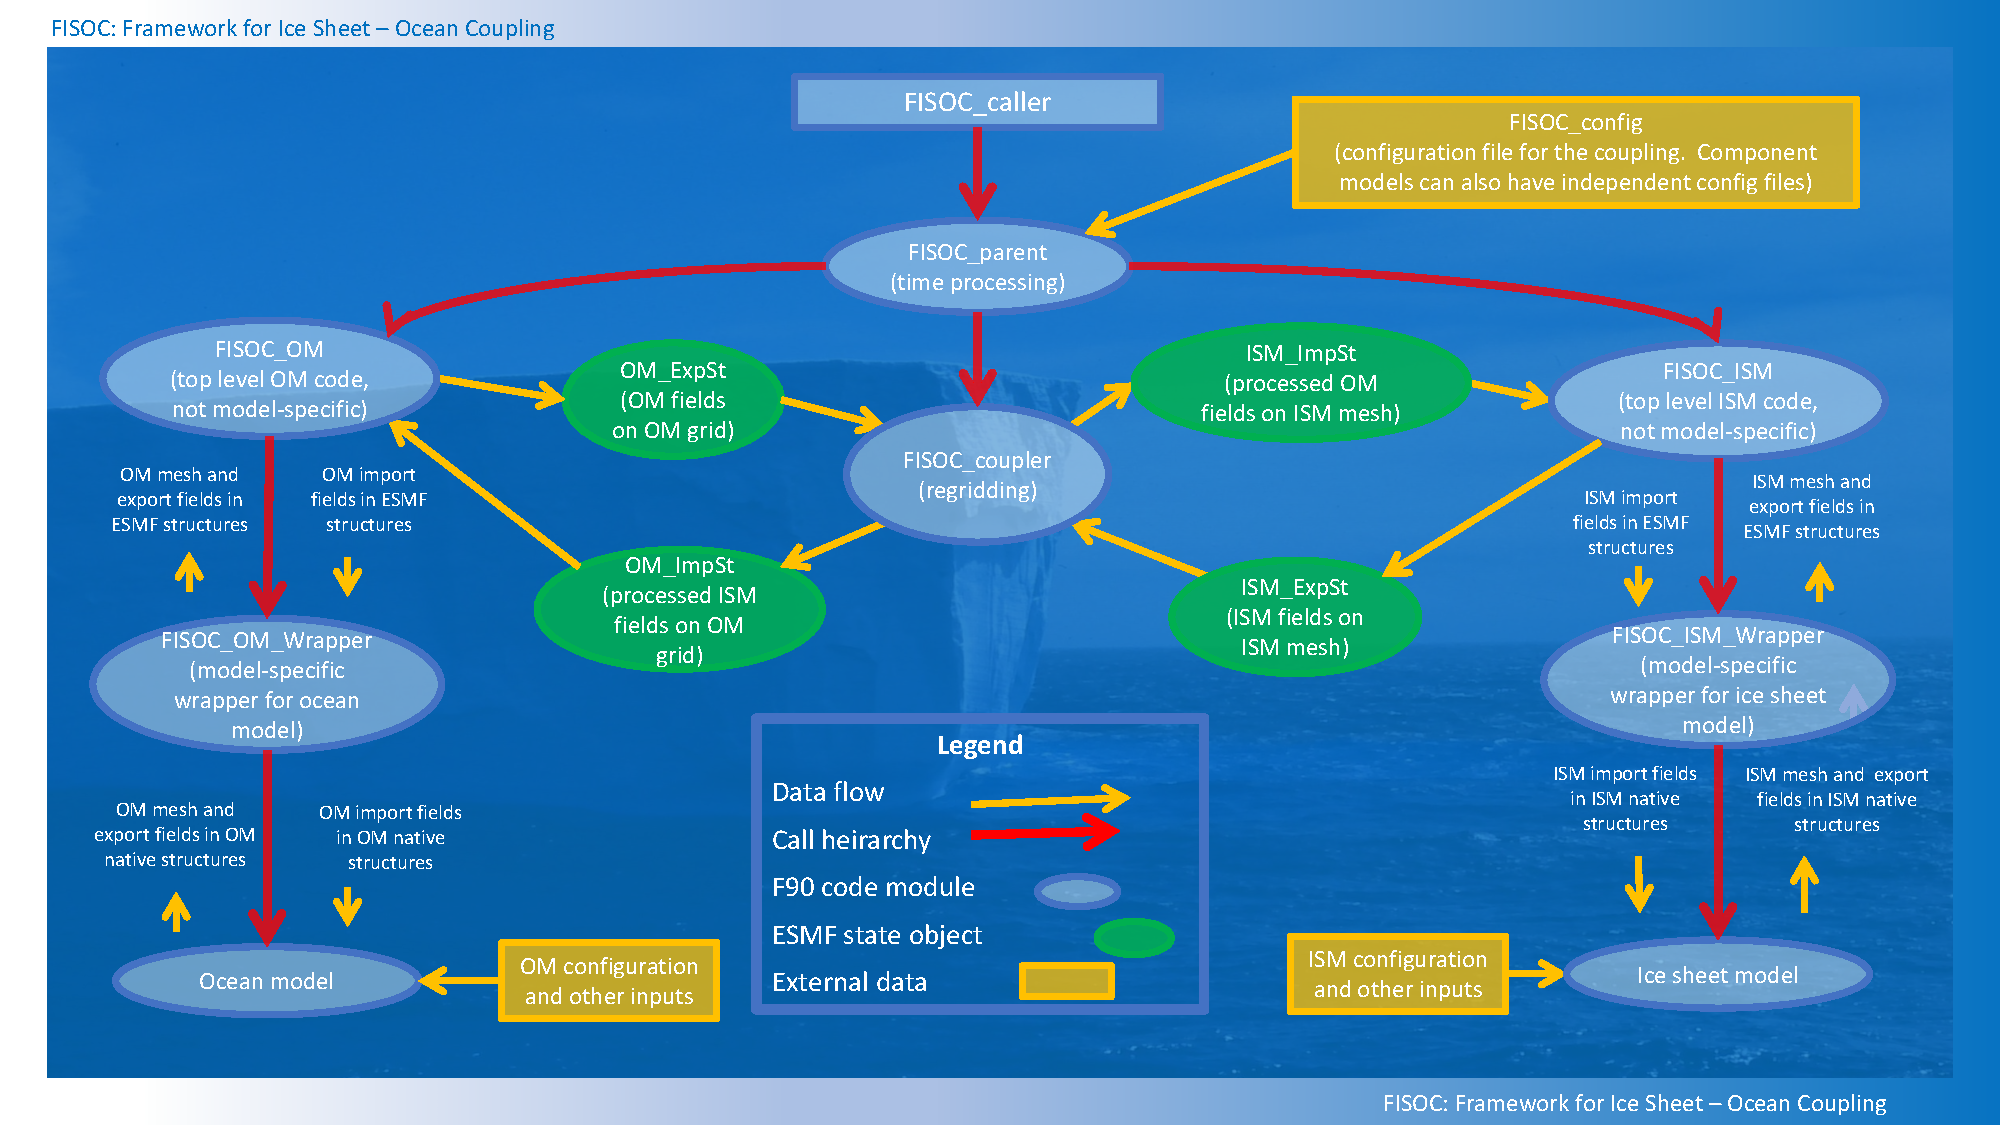
\includegraphics[width=17cm]{FISOC_structure2.pdf}
%    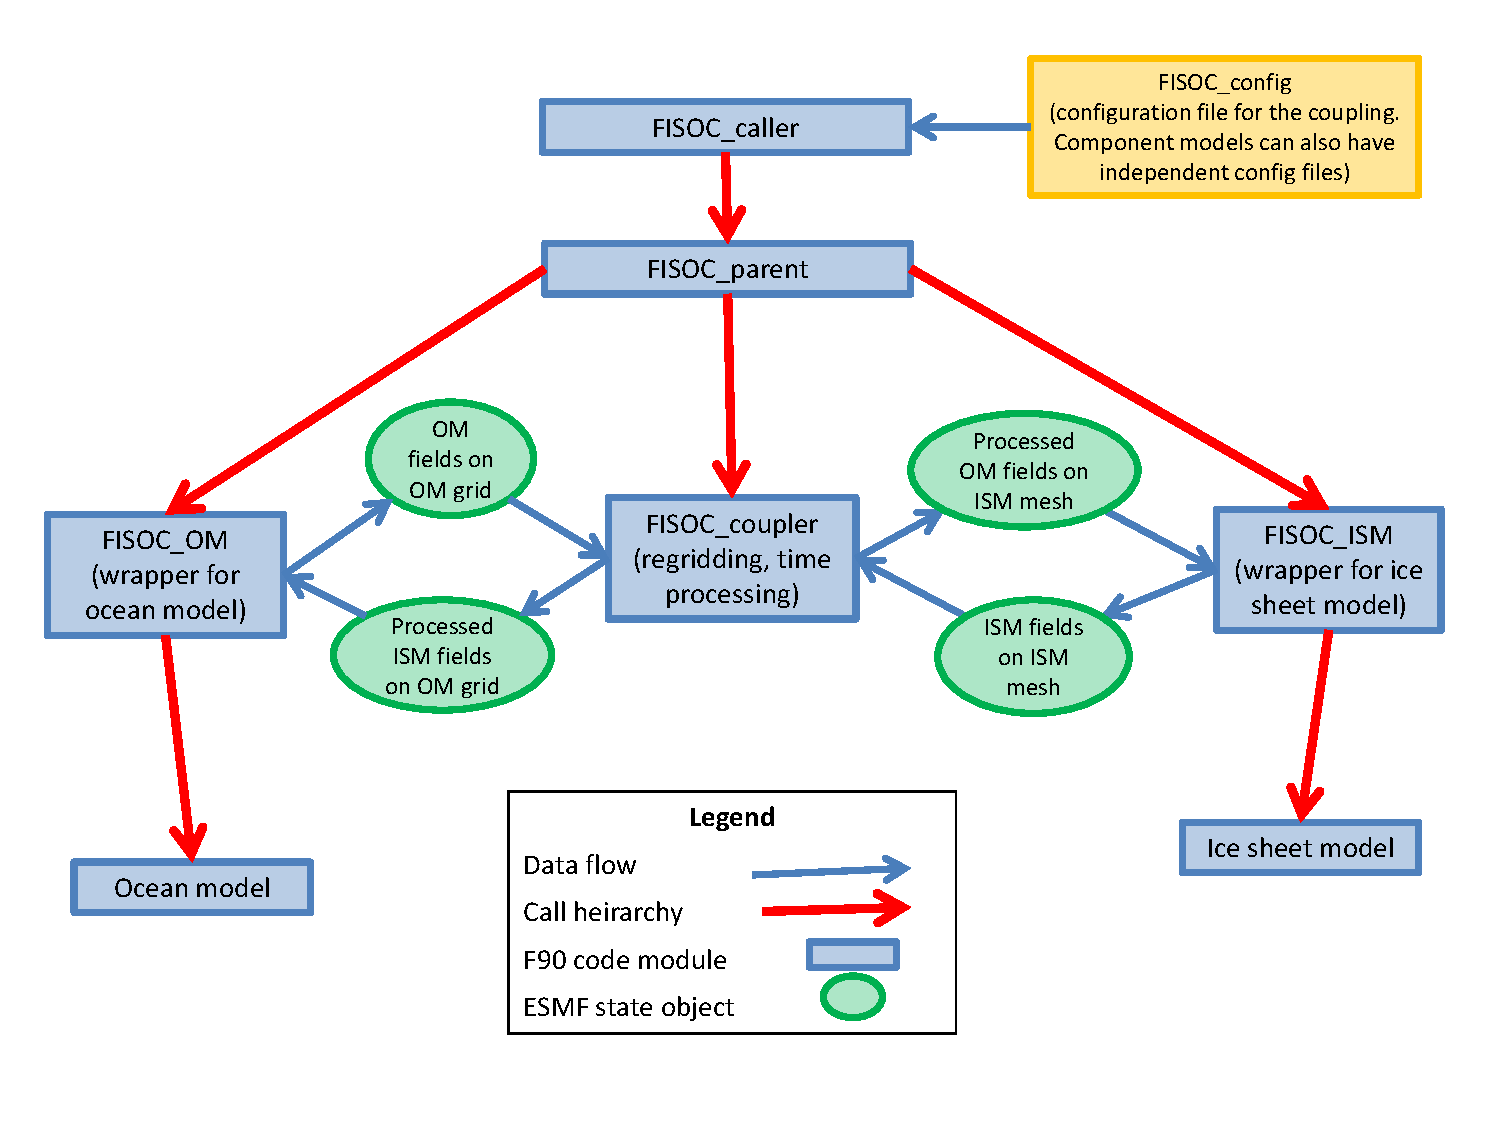
\includegraphics[width=17cm]{FISOC_structure.pdf}
  \end{center}
  \caption{FISOC code and data structures.}
  \label{fig:codeStruct}
\end{figure}



\subsection{Incorporating new OM or ISM components}

FISOC is designed such that the only code developments for new components should be the creation 
of model-specific wrappers: \\
FISOC\_OM\_Wrapper\_XXX.f90 \\
 FISOC\_ISM\_Wrapper\_XXX.f90 \\
where XXX should be replaced by the component's name.

The new wrapper must contain a Fortran module with a fixed name 
and fixed interface for the key init, run and finalise methods. 
The precise requirements are not documented here as they may evolve 
during continued development.  
It is recommended to view an existing wrapper, especially the 
PUBLIC routines.

The following copy from the OM dummy wrapper (7/12/2017) gives 
an example:

\begin{lstlisting}
MODULE FISOC_OM_Wrapper

  USE ESMF
  USE FISOC_utils_MOD

  IMPLICIT NONE

  PRIVATE

  PUBLIC :: FISOC_OM_Wrapper_Init_Phase1,  FISOC_OM_Wrapper_Init_Phase2,  &
       FISOC_OM_Wrapper_Run, FISOC_OM_Wrapper_Finalize, OM_HandleCavity

CONTAINS

...
\end{lstlisting}


Any new OM or ISM component to be used with FISOC must first be ESMF compliant.  This basically 
means that it should have an initialise, run and finalise routine, and that the developer can 
provide the component's grid and variables in ESMF compatible formats through the new wrapper.
The ESMF web site provides further documentation.
\url{https://www.earthsystemcog.org/projects/esmf/}

If it is found that changes to other aspects of the FISOC code are required, this should be 
implemented in collaboration with the FISOC core developers.

Please implement your developments in a new branch in the FISOC repository. 
Request a merge to master when you are happy that it is stable. 




\subsection{Coding practices}

A new component wrapper  should be in a Fortran 90 module.  
All modules should contain the ``implicit none'' statement at the top (immediately after any 
``USE'' statements).  This property will be inherited by all procedures in the module.

FISOC modules have the private attribute, with only required procedures being 
made public. 
New model-specific wrapper modules should ensure that the initialise, run and finalise 
subroutines are public. 



\subsubsection{Error handling}

ESMF provides defensive error handling, with error codes and error messages passed up the 
call stack. 
FISOC implements ``fail-fast'' error handling, with errors generally being considered 
fatal. 
Exceptions to this may be made where it is safe to do so (e.g. where a default value can be 
used in the event of  failure to find a config parameter).
All calls to ESMF routines have return codes checked immediately, and errors logged.
If components (OM or ISM) provide a return code or error code, 
this should be checked by the component wrapper.

Note that many FISOC subroutines contain a return code, but these are mostly not used in 
practice.  Since errors are generally considered instantly fatal in FISOC, execution will 
generaly not get as far as returning a failure code. 
If a more defensive rather than fail-fast approach is adopted in the future these return 
codes can be used.



\subsection{Configuration options}

The configuration file must be named ``FISOC\_config.rc''.  
It is compatible with ESMF config methods.  
An ESMF\_config object is automatically created from this file at run time.
This object is always named ``FISOC\_config'' in the FISOC code.
New model-specific parameters needed by the new wrappers may be 
introduced to the config file and can be accessed 
within the model-specific wrapper at run time, via  ``FISOC\_config''. 
No further coding is needed for this functionality.
See existing model-specific wrappers (e.g. FISOC\_ISM\_Wrapper\_Elmer.f90) 
for examples of this.

The master list of standard FISOC configuration options is contained in 
FISOC/doc/FISOC\_emacsMode.asc and in Section~\ref{sec:config} of this 
manual. 
When new standard configuration options are added during development, they 
should also be added to both the emacsMode file and  
Section~\ref{sec:config} of the manual.


\subsubsection{Default values and derived attributes}

The config file is intended to avoid duplication of information.  
In the case of configuration options that can be derived from other 
configuration options, their derivation is hard coded into 
FISOC\_utils.f90 (see FISOC\_ConfigDerivedAttribute interface) 
rather than adding redundant parameters to the config file.
It is recommended (though not strictly required) that further developments 
also follow this approach. 

Note that the approach of derived attributes can be used to hard code a 
default value for an attribute that is in essence not a derived attribute. 
Using the derived attribute subroutines as a wrapper in which to hard 
code a default value has the benefit of entering the hard coded value 
only at one location rather than each time the attribute is accessed 
from the config object.

%\subsection{ISM wrapper}

%\subsection{OM wrapper}

%\section{Future developments}



\clearpage

\appendix

\section{Pre-requisite installation notes}
\label{app:A}
The following commands worked to install NetCDF and ESMF on a Linux Mint system in 2015 
in a suitable configuration for use with FISOC. 
Some pre-requisites for netcdf were also installed.
The system already had a working OpenMPI installation.



\begin{lstlisting}[language=bash]


# instructions on installing ESMF can be found here:
# http://www.earthsystemmodeling.org/esmf_releases/last_built/ESMF_usrdoc/node9.html

# netcdf instructions
# http://www.unidata.ucar.edu/software/netcdf/docs/netcdf-install.html

cd /somewhere/to/download/and/compile/source/code

sudo apt-get install m4

wget ftp://ftp.unidata.ucar.edu/pub/netcdf/netcdf-4/zlib-1.2.8.tar.gz
tar -xzf zlib-1.2.8.tar.gz 
cd zlib-1.2.8
 ./configure --prefix=/usr/local/
 make check
 sudo -E make install
cd ..

wget ftp://ftp.unidata.ucar.edu/pub/netcdf/netcdf-4/hdf5-1.8.13.tar.gz	
tar -xzf hdf5-1.8.13.tar.gz 
cd hdf5-1.8.13
 # Note the O0 flag in the next line.  The default is O3, 
 # which is strong optimisation.  This can result in failed 
 # checks on some systems.
 CFLAGS="-O0 -fPIC" CC=mpicc CXX=mpiCC FC=mpif90 ./configure --prefix=/usr/local/ --with-zlib=/usr/local  --enable-fortran --enable-parallel --enable-shared
 make check
 sudo -E make install
cd ..

# note that netcdf fortran library is now compiled from a 
# seperate source from the main netcdf c library. Install 
# the c library first, and make sure to create the shared
# object file. 
wget ftp://ftp.unidata.ucar.edu/pub/netcdf/netcdf-4.3.3.tar.gz
tar -xzf netcdf-4.3.3.tar.gz 
cd netcdf-4.3.3/
 LIBS=-ldl CC=mpicc CXX=mpiCC FC=mpif90 CPPFLAGS=-I/usr/local/include/ LDFLAGS=-L/usr/local/lib/  ./configure --prefix=/usr/local --enable-parallel 
 make check
 sudo -E make install
cd ..

wget ftp://ftp.unidata.ucar.edu/pub/netcdf/netcdf-fortran-4.4.2.tar.gz
tar -xzf netcdf-fortran-4.4.2.tar.gz 
cd netcdf-fortran-4.4.2
 LIBS=-ldl CC=mpicc CXX=mpiCC FC=mpif90 LDFLAGS=-L/usr/local/lib/ CPPFLAGS="-I/usr/local/include -DUSE_NETCDF4"  ./configure --prefix=/usr/local
 make check
 sudo -E make install
cd ..

# convenient viewer for contents of netcdf files (not essential)
sudo apt-get install ncview

# ESMF requires ESMF_DIR and probably other environment variables.  
# These can be set at the command line or, for example, in your 
# .bashrc fileor a local script file.  These might work:
export ESMF_DIR="/top/level/directory/for/esmf/"
export ESMF_NETCDF="split"
export ESMF_NETCDF_INCLUDE="/usr/local/include"
export ESMF_NETCDF_LIBPATH="/usr/local/lib"
export ESMF_COMM="openmpi"
export ESMF_PIO="internal"
                                                                                                              
wget downloads.sourceforge.net/project/esmf/ESMF_6_3_0r/ESMF_6_3_0rp1/esmf_6_3_0rp1_src.tar.gz
tar -xf esmf_6_3_0rp1_src.tar.gz
cd esmf 
 make check
 sudo -E make install
cd ..

# In order to actually use ESMF you must set the environment 
# variable ESMFMKFILE.  If you didn't use environment 
# variables to specify the install location this make file 
# will probably end up somewhere like this:
export ESMFMKFILE="$ESMF_DIR/DEFAULTINSTALLDIR/lib/libO/Linux.gfortran.64.openmpi.default/esmf.mk"

\end{lstlisting}
\vspace{10mm}
... or for ESMF version 7.0.0 ...
\begin{lstlisting}[language=bash]
wget https://sourceforge.net/projects/esmf/files/ESMF_7_0_0/esmf_7_0_0_src.tar.gz
tar -xf esmf_7_0_0_src.tar.gz 
\end{lstlisting}
\vspace{10mm}
... or for ESMF version 7.1.0 beta snapshot 14 ...
\begin{lstlisting}[language=bash]
git archive --remote=git://git.code.sf.net/p/esmf/esmf --format=tar --prefix=esmf/ ESMF_7_1_0_beta_snapshot_14 | tar xf -
\end{lstlisting}

\end{document}
